\section{response\_\-handler.h File Reference}
\label{response__handler_8h}\index{response\_\-handler.h@{response\_\-handler.h}}
{\tt \#include $<$string$>$}\par
{\tt \#include $<$sstream$>$}\par
{\tt \#include $<$iostream$>$}\par
{\tt \#include $<$cstdlib$>$}\par
{\tt \#include $<$map$>$}\par
{\tt \#include \char`\"{}../kernel/component.h\char`\"{}}\par
{\tt \#include \char`\"{}../kernel/simulator.h\char`\"{}}\par
{\tt \#include \char`\"{}../simIris/data\_\-types/impl/irisEvent.h\char`\"{}}\par
{\tt \#include \char`\"{}request.h\char`\"{}}\par
{\tt \#include \char`\"{}../util/mc\_\-constants.h\char`\"{}}\par
{\tt \#include \char`\"{}NI.h\char`\"{}}\par
{\tt \#include \char`\"{}cmd\_\-issuer.h\char`\"{}}\par
{\tt \#include \char`\"{}mshr\_\-standalone.h\char`\"{}}\par


Include dependency graph for response\_\-handler.h:\nopagebreak
\begin{figure}[H]
\begin{center}
\leavevmode
\includegraphics[width=420pt]{response__handler_8h__incl}
\end{center}
\end{figure}


This graph shows which files directly or indirectly include this file:\nopagebreak
\begin{figure}[H]
\begin{center}
\leavevmode
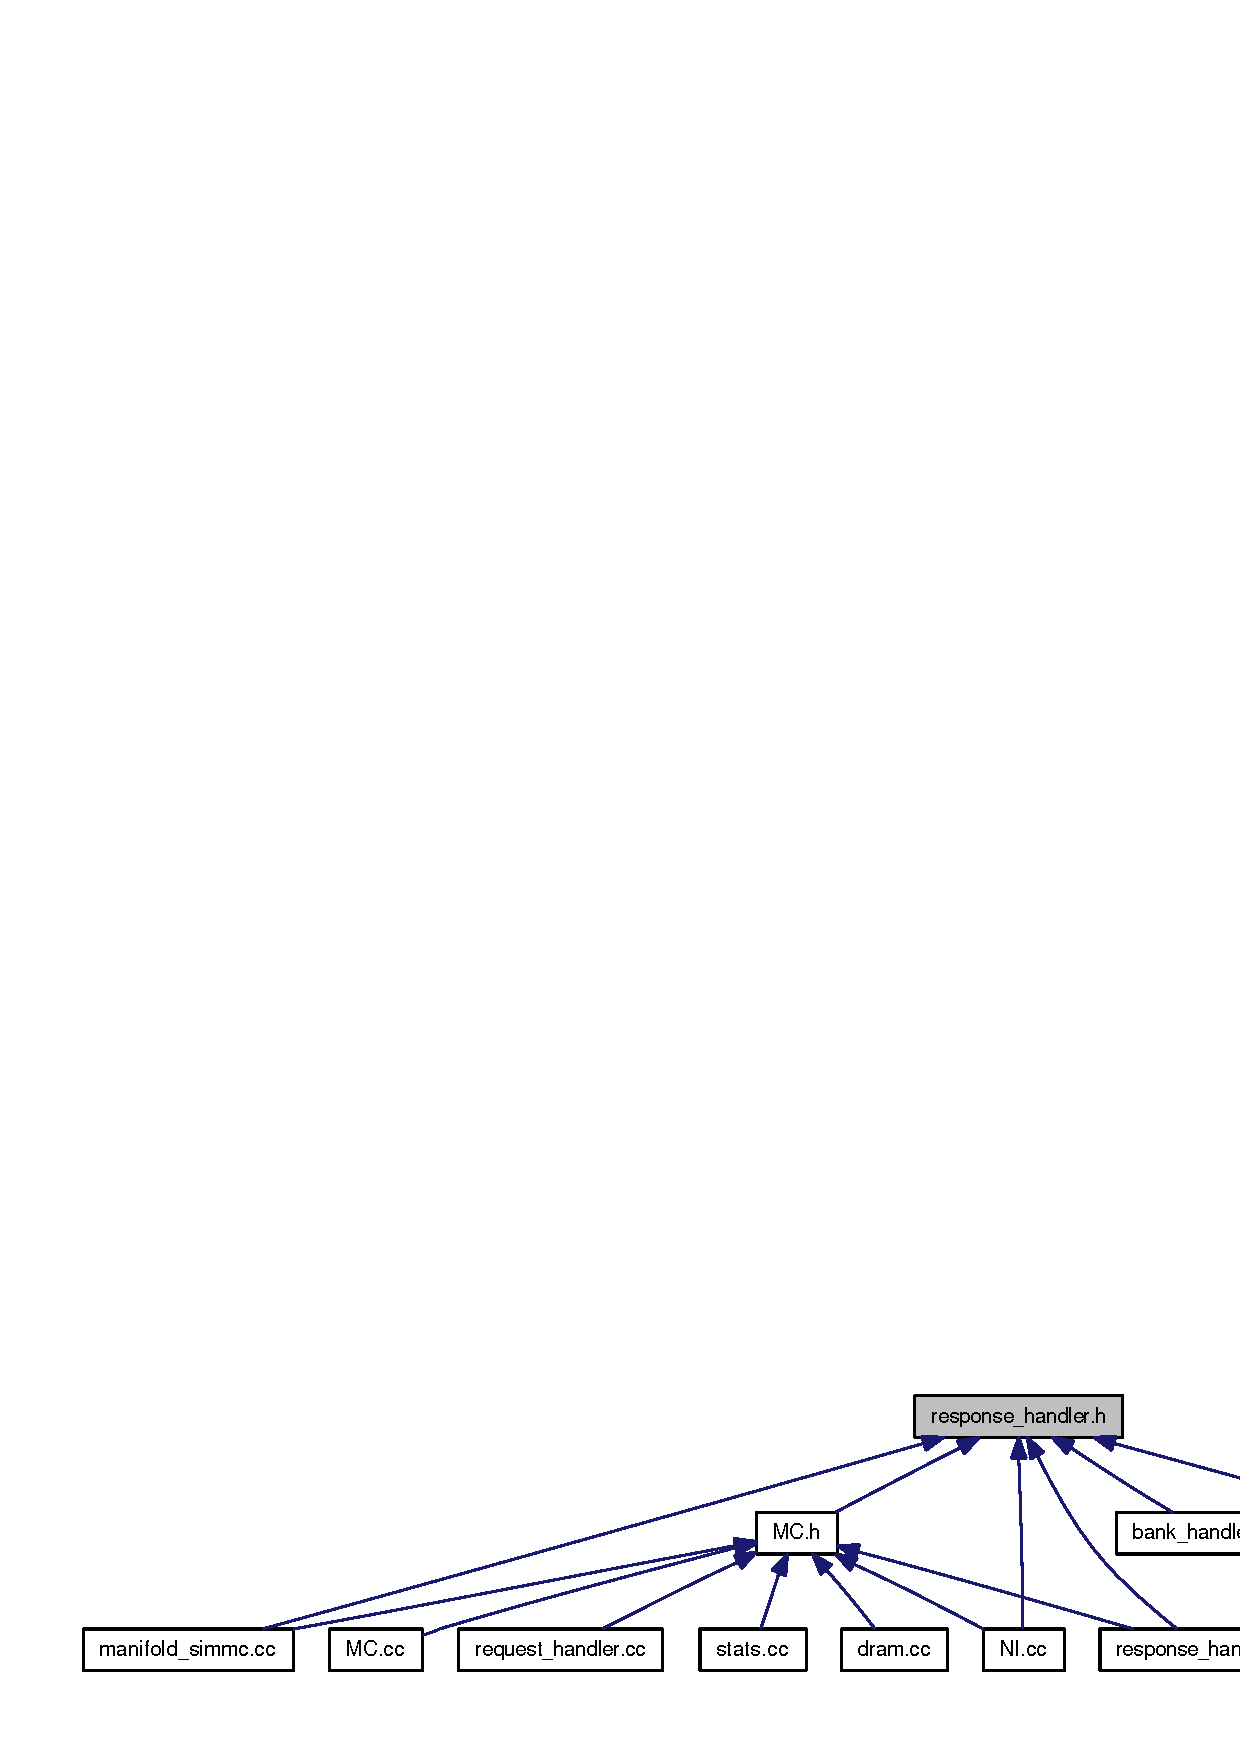
\includegraphics[width=374pt]{response__handler_8h__dep__incl}
\end{center}
\end{figure}
\subsection*{Classes}
\begin{CompactItemize}
\item 
class {\bf ResponseHandler}
\end{CompactItemize}
\subsection*{Variables}
\begin{CompactItemize}
\item 
vector$<$ {\bf MSHR\_\-SA\_\-H} $\ast$ $>$ {\bf mshrHandler}
\end{CompactItemize}


\subsection{Variable Documentation}
\index{response\_\-handler.h@{response\_\-handler.h}!mshrHandler@{mshrHandler}}
\index{mshrHandler@{mshrHandler}!response_handler.h@{response\_\-handler.h}}
\subsubsection[{mshrHandler}]{\setlength{\rightskip}{0pt plus 5cm}vector$<${\bf MSHR\_\-SA\_\-H}$\ast$$>$ {\bf mshrHandler}}\label{response__handler_8h_1fc79726402dfb84d1bfc19aaf5dc776}




Definition at line 46 of file manifold\_\-simmc.cc.

Referenced by GetNextRequest(), main(), and ResponseHandler::process\_\-event().